\subsection{Digital front end}\label{sec:frontend}
The digital front end (DFE) consist of three parts, D flip flop with a NAND and a NOR port. This can been seen in Fig. ~\ref{fig:Global_schematic_DFE_figure}. The D flip flop will synchronise the incoming data and the NAND/NOR gate will up-modulate the signal with the local oscillator in the digital domain. In comparison with the global schematic of the previous group (Appendix: Fig. ~\ref{fig:Global_schematic_previous_group_figure}) the DFE consist of one less D flip flop in the diagram. This will increase the synchronisation of nmos and pmos of the current sources. The DFE works in a high frequency domain and it needs to switch fast. Therefore thin oxide transistors are used. The drawback of this kind of transistors is that they operate at low voltages (max 1.2V), so less power at the output stage. To solve this problem a level shifter is used to increase the power at the output stage. In total 30 DFE circuit and level shifter are made to make the 4 bit power dac, this can be seen in the high level diagram in fig ( This diagram will be in the final report).The level shifter will be described in paragraph ~\ref{sec:levelshifter}. The digital front end will be described in this paragraph.

\begin{figure}[h]
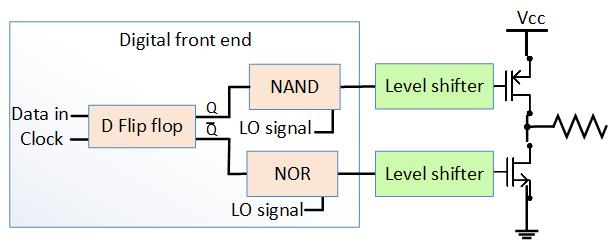
\includegraphics[width=0.5\textwidth]{Global_schematic_DFE.jpg}
\caption{One side of the diagram of the new digital front end.}
\label{fig:Global_schematic_DFE_figure}
\end{figure}

\subsubsection{D flip flop}\label{sec:frontend}
A D flip flop will be used to synchronise the incoming thermometer coded data to ensure that the transistors of the output stage switch at the same time. There are a couple of challenges that are important to take into account when designing a D flip flop, for example the operation speed and the transition time of the output at the rising clock.
A flip flop can be made in different ways. The two main technologies are in CMOS and CML. The CMOS design is relatively less complex in compare to CML, but in CML there are more parameters that can be modified to tune the output. In this project the CMOS design is used, because it is less complex, single-ended and it can be realised in a short time period. 

The CMOS circuit of previous group is been used as basic circuit. ~\cite{coursebook} -~\cite{powerdac}. The old schematic can been seen in the appendix Fig.~\ref{fig:D_flip_flop_ previous_group_figure}. The new schematic consist of 32 transistors and is showed in Fig.~\ref{fig:D_flip_flop_schematic_figure}. There are three changes made in compare with the old schematic. The first changes is that a second output is been added to flip flop, as mentioned before to reduce one flip flop in the total schematic. The second changes is a cmos switch is added to improve the synchronisation between the output and the input. The last changes is that the sizes of the nmos and the pmos transistors are changed, to reduce the delay of the output. The size of the nmos and pmos will be further discussed, first the basic principle of a D flip flop will be explained. 

\begin{figure}[h]
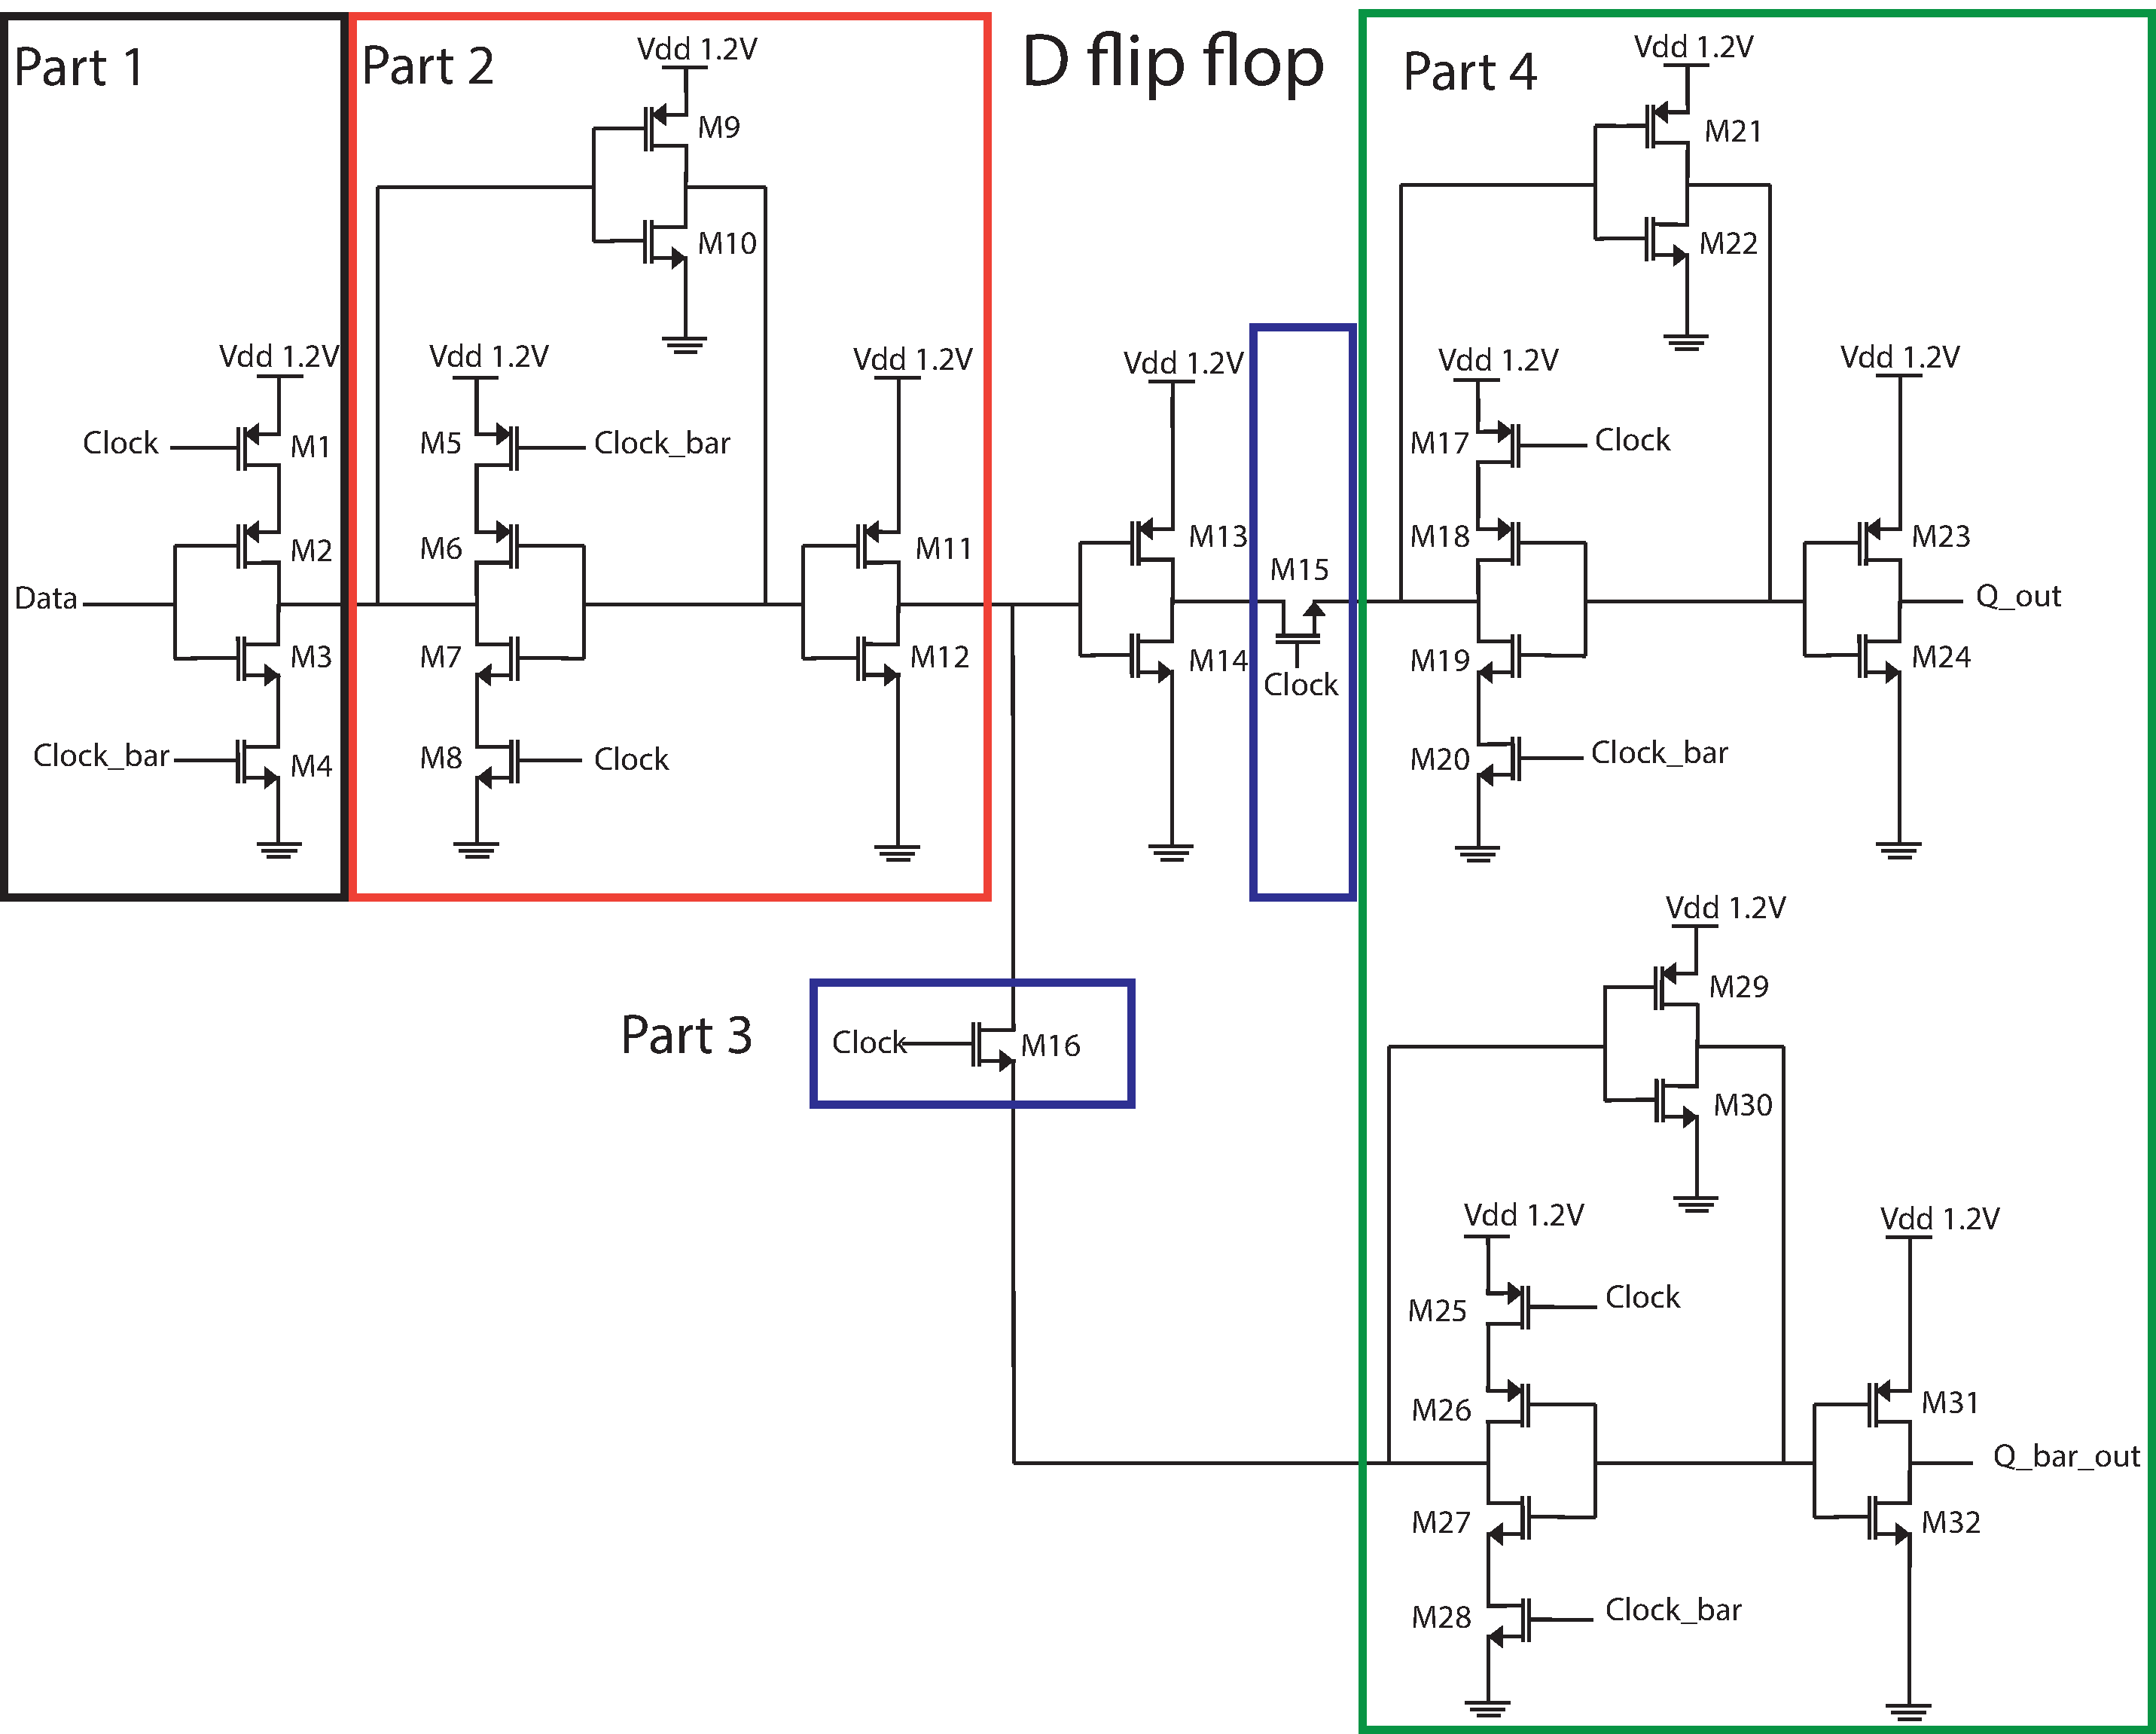
\includegraphics[width=0.5\textwidth]{D_flip_flop_new_schematic.pdf}
\caption{The improved D flip flop schematic.}
\label{fig:D_flip_flop_schematic_figure}
\end{figure}

The D flip flop works with a master-slave principal. The master will set the data on the rising clock and it will hold the data until the clock is low. The slave will copy the data when the clock is high and hold the data when the clock is low.

To explain this principle, the schematic can be divided into four parts, settle time of the data, master latch, two switches and slave latch. In the first part the data will be set when the clock is low. The second part, the master will follow the signal of the first part when the clock is low and hold the data when the clock is high. In the third part the switches will be closed when the clock is high. The slave latch(part 4) can set the data and when the clock is high it will hold the data.
 
The size of the pmos and nmos of part one, two and four are the same. The size of the nmos is set on 50nmx90nm (length x width). The length of the pmos is the same, but the width of the pmos is determined with a parameter sweep to get the lowest delay of transition. In the parameter sweep the clock frequency is set on 1 GHz and the data frequency is set on 500MHz. The results are showed in the appendix in Fig.~\ref{fig:parametersweep_changing_w_low_to_high_figure} and Fig.~\ref{fig:parametersweep_changing_w_high_to_low_figure}. The optimal width of the pmos is 180nm. It has the best average delay of transition from high to low and low to high.

With the sizes of the master and slave set, the width of the switching nmos (part 3) needs to be determined. This is also done with a parameter sweep with the same clock and data frequency. The results of the parameter sweep are shown in Fig.~\ref{fig:Parameter_sweep_changing_w_of_the_swiching_nmos_high_to_low_figure} and Fig.~\ref{fig:Parameter_sweep_changing_w_of_the_swiching_nmos_low_to_high_figure} in the appendix. The optimal value of the width is 360nm. The results of this value is compared with the previous schematic and is shown in Fig.~\ref{fig:Comparison_old_schematic_and_new_schematic_low_figure} and Fig.~\ref{fig:Comparison_old_schematic_and_new_schematic_high_figure}. The delay of transmission is reduced 18.5ps for Q and 3.64ps for Q bar when the output goes from high to low and when the output goes from low to high the delay is reduced with 20.4ps for Q and 13.5ps. With this result the synchronisation will be improved.

\begin{figure}[h]
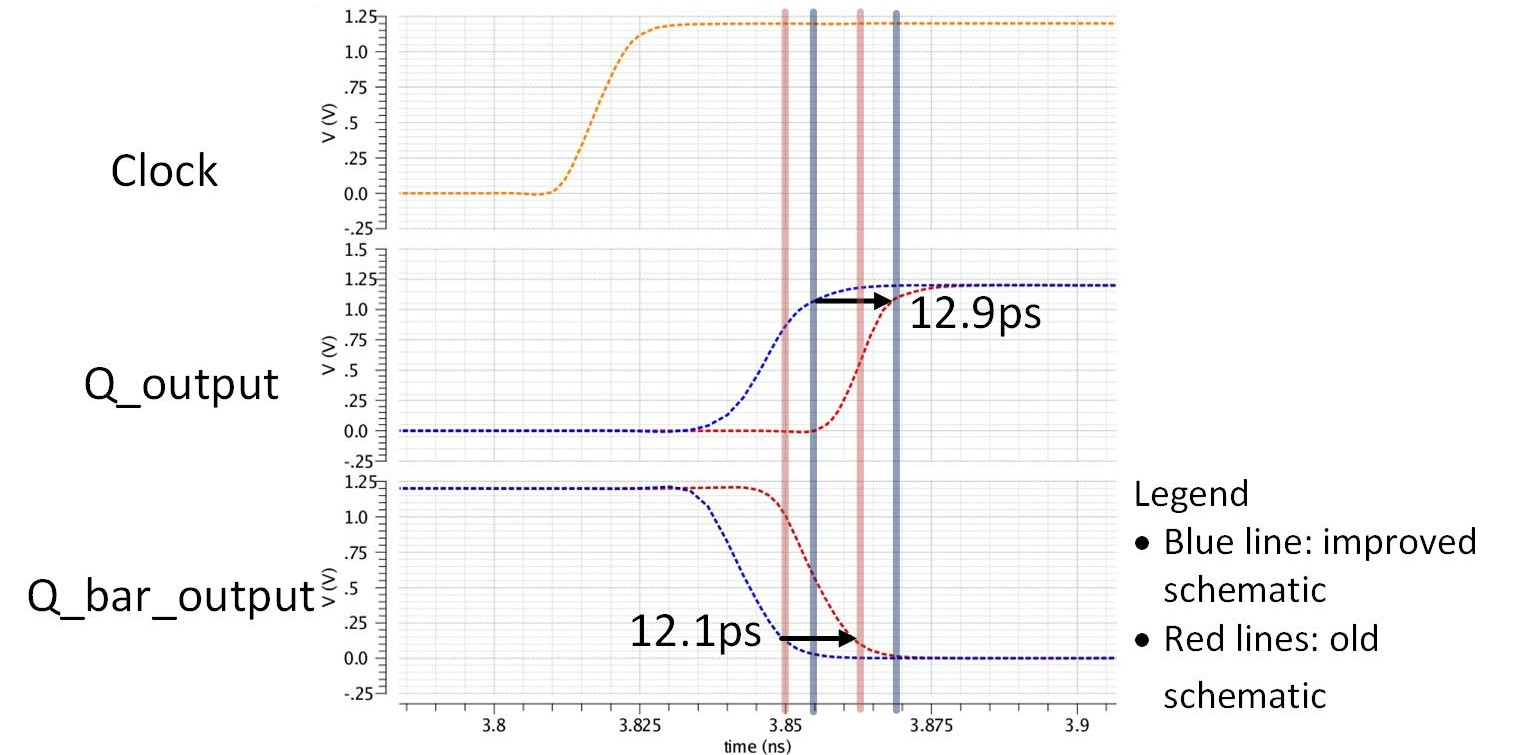
\includegraphics[width=0.5\textwidth]{Comparison_old_schematic_and_new_schematic_high.jpg}
\caption{Comparison of the delay of transition between the old schematic and the new schematic when the data is high }
\label{fig:Comparison_old_schematic_and_new_schematic_high_figure}
\end{figure}

\begin{figure}[h]
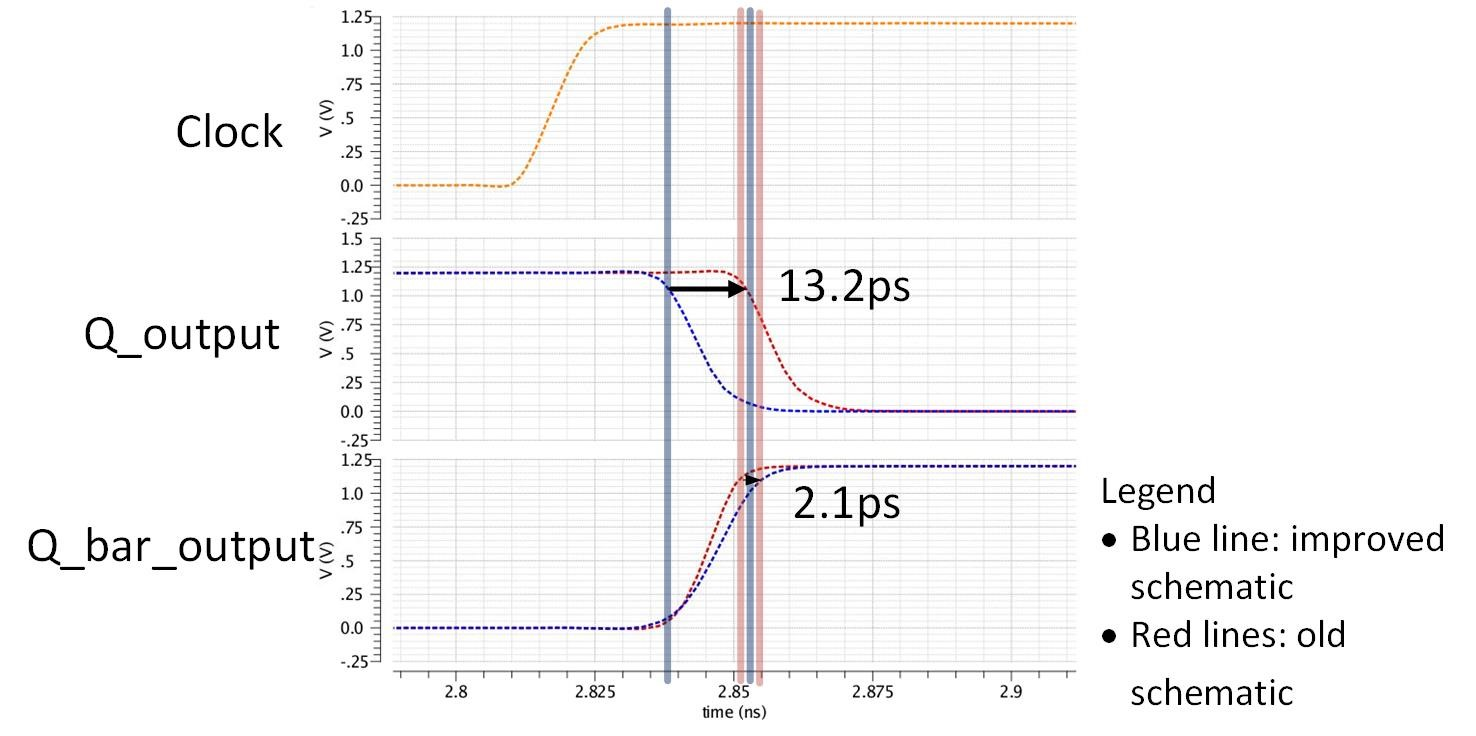
\includegraphics[width=0.5\textwidth]{Comparison_old_schematic_and_new_schematic_low.jpg}
\caption{Comparison of the delay of transition between the old schematic and the new schematic when the data is low.}
\label{fig:Comparison_old_schematic_and_new_schematic_low_figure}
\end{figure}

With all the transistors size known the critical point can be measured. The minimal time that the data needs to be set is 40ps before the clock is high. The transition delay of Q is 26.46ps and Q bar is 20.7ps when the data is high. When the data is low the delay of Q is 22ps and Q bar is 25ps. This is shown in Fig.~\ref{fig:Critical_values_data_high_to_low_figure} and Fig. ~\ref{fig:Critical_values_data_low_to_high_figure}. 

\begin{figure}[h]
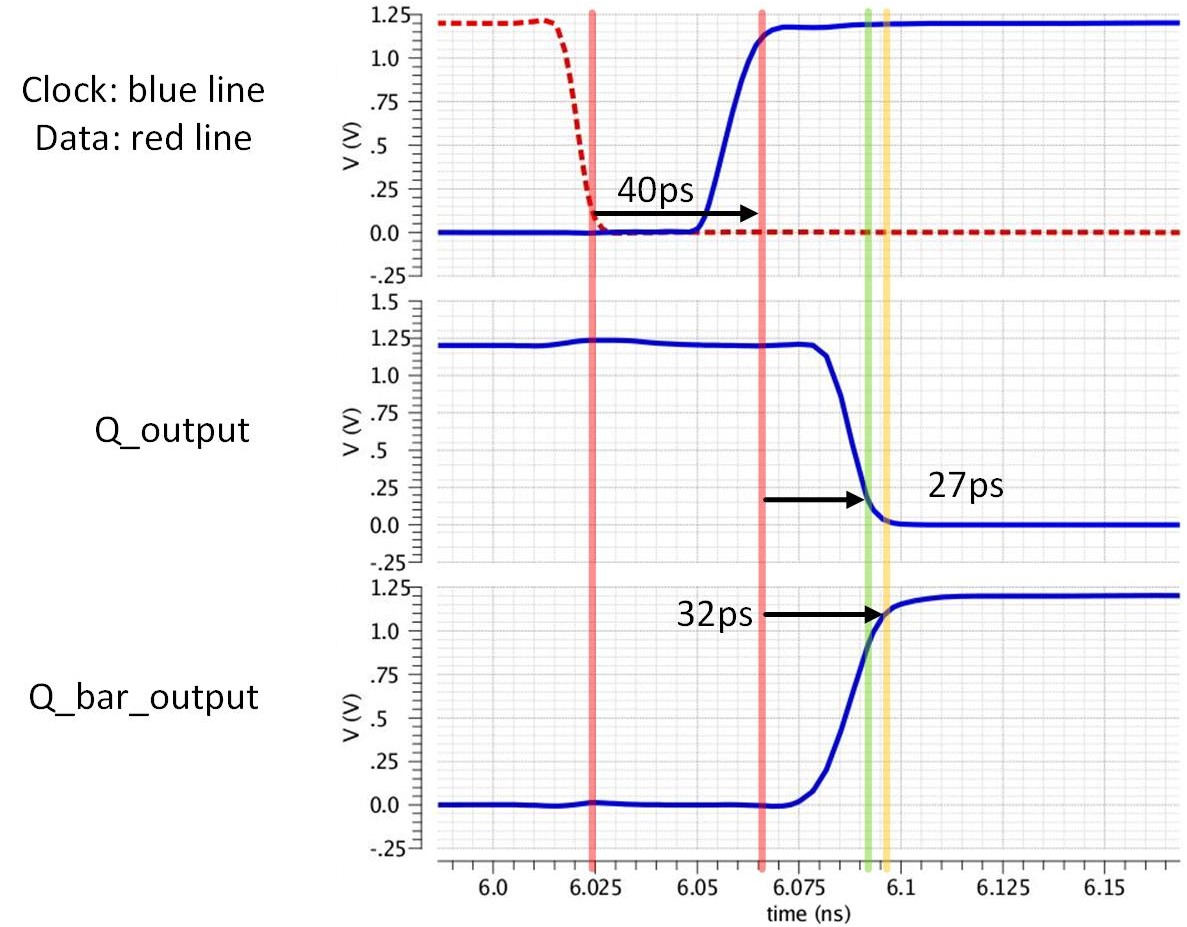
\includegraphics[width=0.5\textwidth]{Critical_values_data_high_to_low.jpg}
\caption{The critical values when the data goes from high to low}
\label{fig:Critical_values_data_high_to_low_figure}
\end{figure}

\begin{figure}[h]
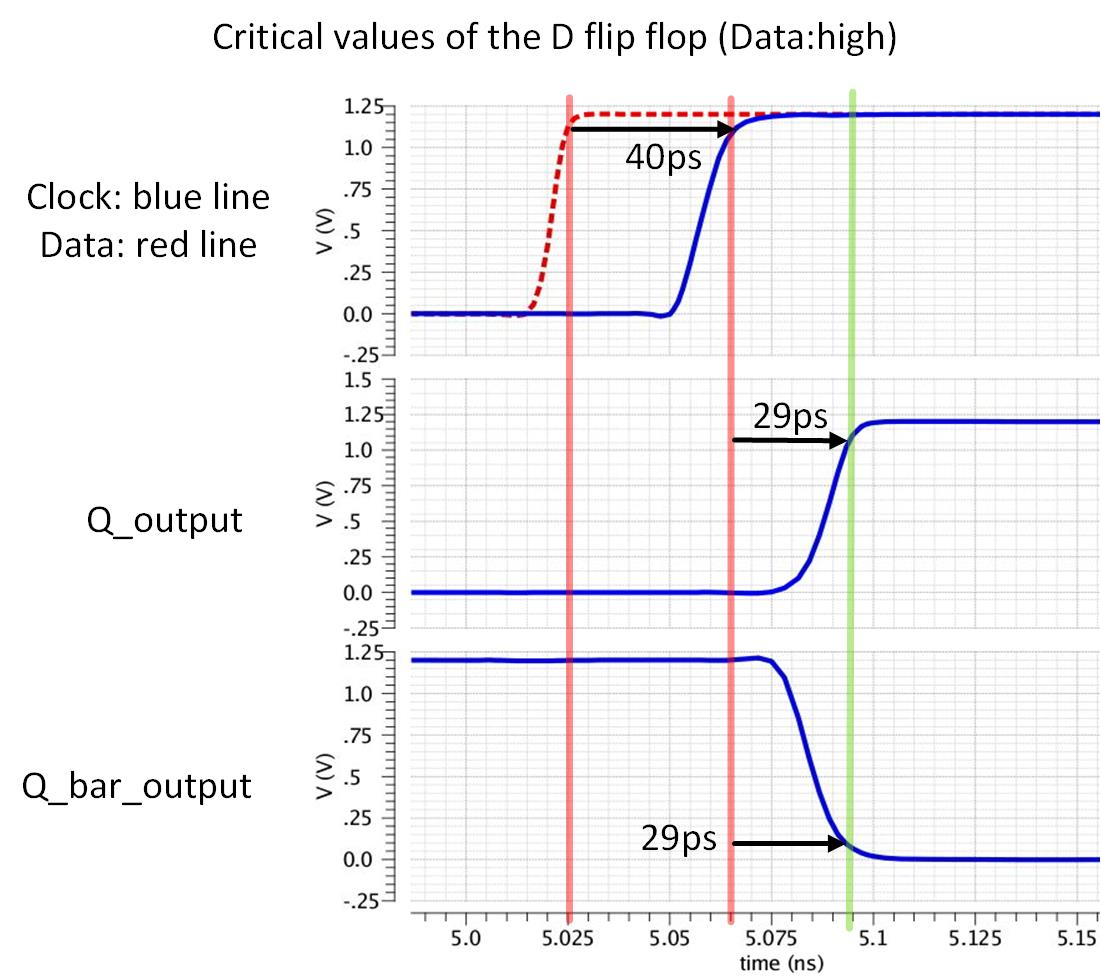
\includegraphics[width=0.5\textwidth]{Critical_values_data_low_to_high.jpg}
\caption{The critical values when the data goes from high to low.}
\label{fig:Critical_values_data_low_to_high_figure}
\end{figure}

\subsubsection{NAND/NOR gate}\label{sec:frontend}
The NAND and NOR will up-modulate the local oscillator signal (LO) with the data from the D flip flop. This will happen in the digital domain with an LO signal of 2Ghz square wave.
The design of a NAND and NOR is shown in Fig.~\ref{fig:NAND_schematic_figure} and Fig.~\ref{fig:NOR_schematic_figure}.

\begin{figure}[htp]
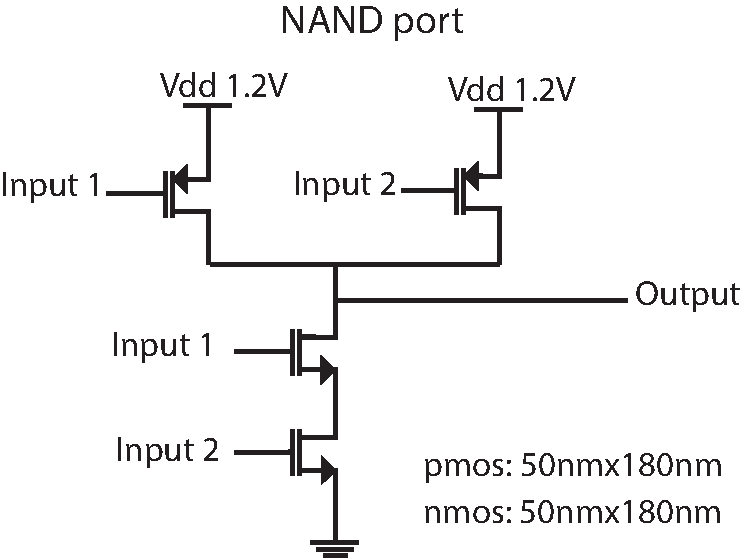
\includegraphics[width=0.4\textwidth]{NAND_schematic.pdf}
\caption{The schematic of the NAND port.}
\label{fig:NAND_schematic_figure}
\end{figure}

The NAND port has two pmos in parallel and 2 nmos in series. In a normal cmos inverter the size of the pmos is 2 times larger than the nmos. In this situation two nmos transistors are in series, so the width of the nmos needs to be 2 times larger to get an equal resistance. The two pmos remains the same value as in a normal cmos inverter, thus the nmos and pmos have the same size of transistor of 50nmx180nm (length x width).

\begin{figure}[htp]
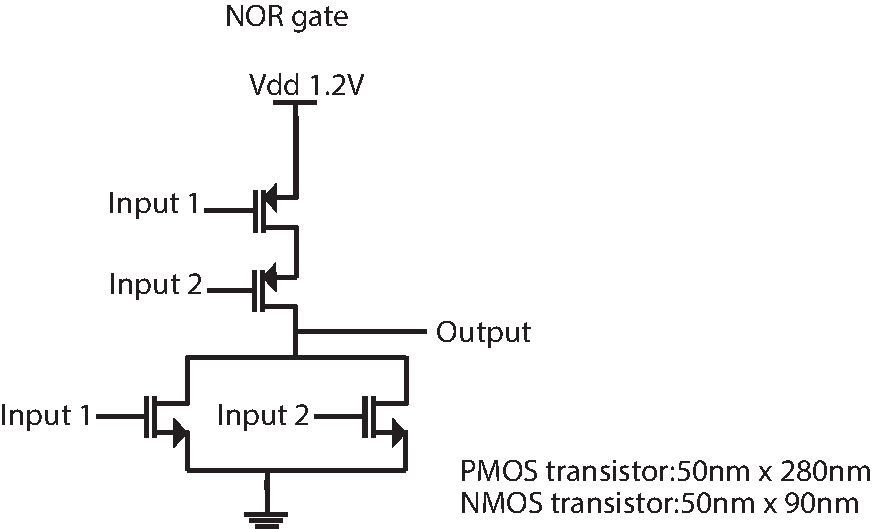
\includegraphics[width=0.35\textwidth]{NOR_schematic.pdf}
\caption{The schematic of the NAND port.}
\label{fig:NOR_schematic_figure}
\end{figure}

The NOR port has two pmos in serie and 2 nmos in parallel. The width of the PMOS is 4 times larger than the nmos, because the two pmos are in serie and of the relation between the nmos and pmos mobility factor. The size of the nmos will be 50nmx90nm (length x width) and pmos 50nm0x360nm (length x width).
